% !TeX root = ../thuthesis-example.tex

\chapter{Discussion and future perspectives}

\begin{figure}[b]
    \centering
    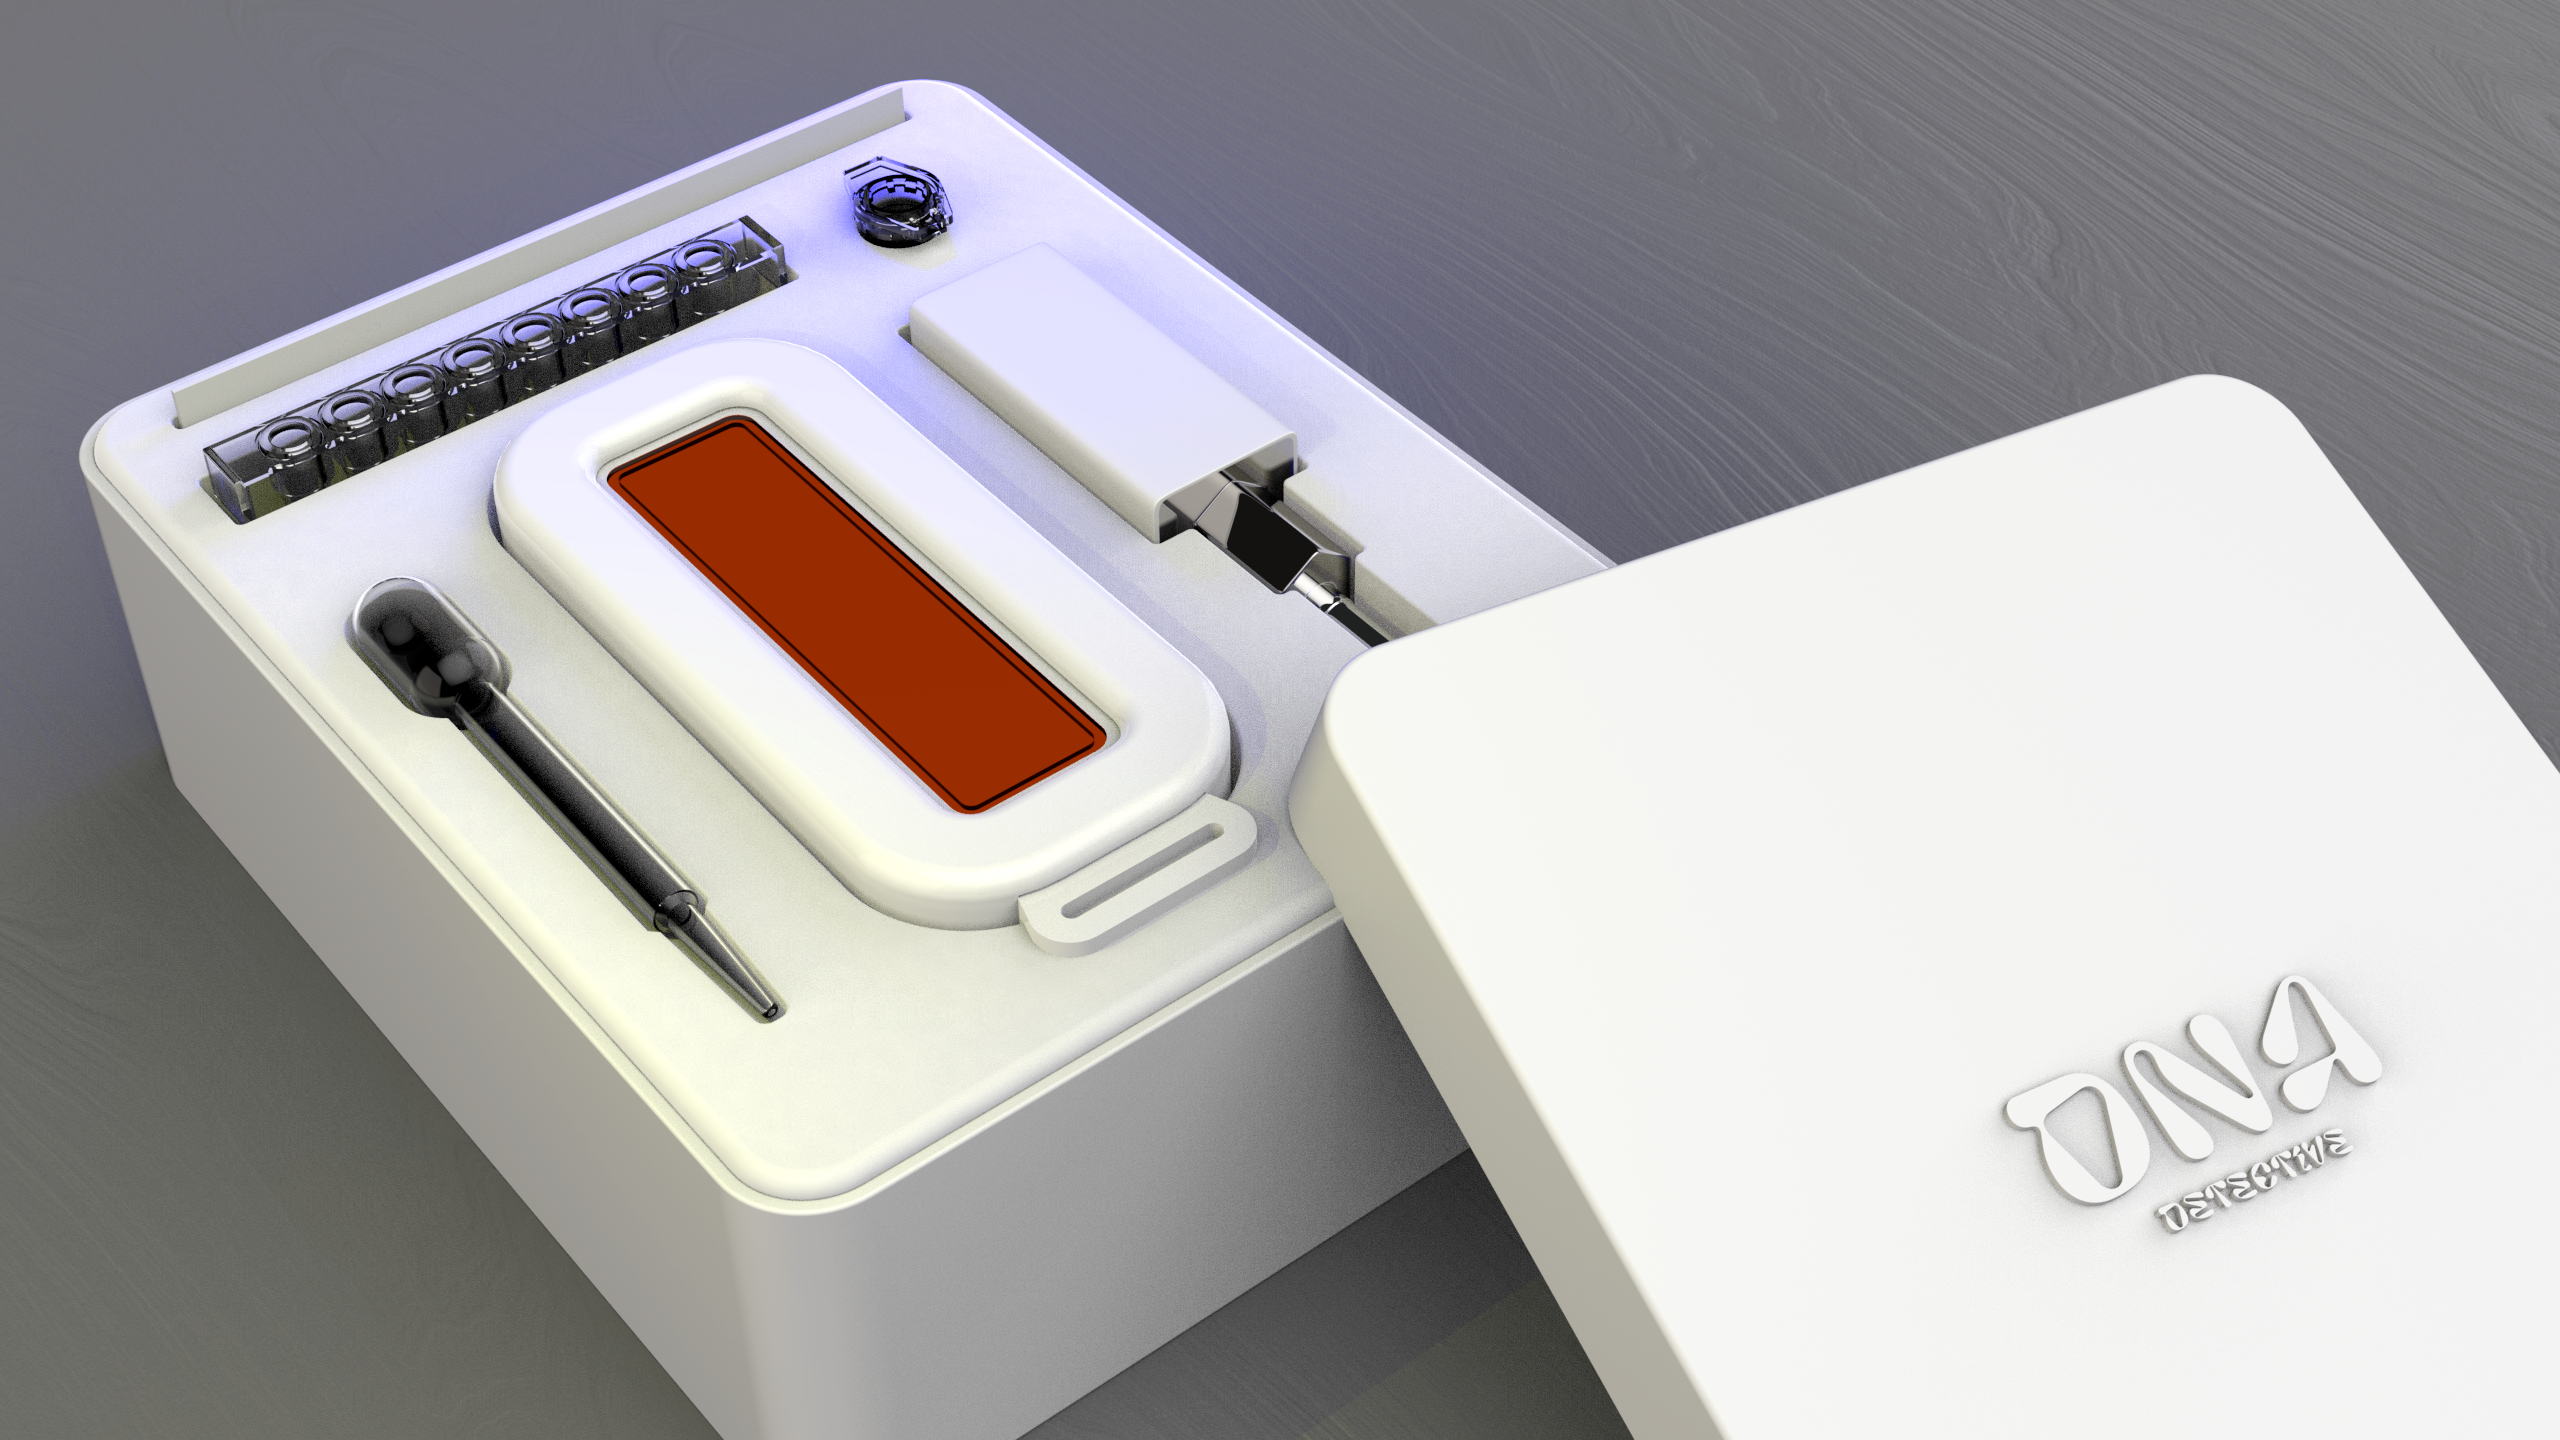
\includegraphics[width=0.95\textwidth]{figures/kit simulation.png}
    \caption{Simulation of the final kit. Image generated by Blender using the 3D models in the GitLab repository of this project\cite{francisco_javier_quero_lombardero_open_2021}.}
    \label{Final kit}
\end{figure}

During this thesis, we have described the design and successful implementation of a series of biotechnological and hardware tools that take the simplicity and affordability of infectious disease detection to the next level. In addition, both protocols and designs have been registered under open source licenses, allowing anyone to replicate the system locally.
    
Although future additional tests are needed (with better quality clinical samples) the performance of both CoronaDetective and water bath reactions has been satisfactorily demonstrated throughout this thesis. Furthermore, the possibility of lyophilizing the reactions to vastly increase their room temperature stability has been described. With a price of \$2 for the reactions and \$5 for the hardware, being easy to use and replicate, not needing refrigeration, being portable and presenting the robustness to false positives of a PCR, this technology presents itself with a great potential to be a game-changer in the low resource diagnostics panorama.
 
 \newpage   
The real-time lamp kit described in the last part of Chapter 4, while still requiring future adjustments, has enormous potential to enable the quantitative analysis of nucleic acid amplification at the price of ~\$50. This cost represents three orders of magnitude of improvement over previous commercial alternatives and opens a massive window of possibilities for both research and diagnostics in LMICs.

However, future work is still needed. To achieve a real impact, we must gain recognition for the use of this technology as an \emph{in vitro} diagnosis certified tool. In this topic, we have an advanced conversation with the local regulatory agencies in Ghana, the Noguchi institute and the local Ghana FDA agency. In our opinion, the next important step on the road to certifying and deploying the technology involves creating a kit in the form of a final product containing all the components necessary to carry out the detection protocol. This kit should package inside the hardware, reactions, and other materials an end-user requires, such as affordable liquid handling solutions or a simple and intuitive user manual (Figure 5.1). Once an initial batch of the kit is produced the system will be ready to enter in the trials to get the local \emph{in vitro} diagnosis certification.
        
Nevertheless, the largest potential to support the development of LMICS is stablishing a local production of the technology. The reactions are simple, using a single enzyme, which is crucial in making production possible in the field. Early in the pandemic, we contributed to create the Reclone online collaborative network \cite{recloneorg_reagent_nodate} in which researchers around the world can share and review protocols for enzyme production at low resources settings. To start exploring the local production of enzymes, many researchers have been exploring ways of harvesting the potential of synthetic biology to create easy protocols to produce and purify Bst polymerases on the field\cite{rivera_recombinant_2020}. If Bst can potentially be manufactured on the ground, this would allow LMICs to gain enormous industrial autonomy from the main producing areas of the planet (Europe, the United States and China), alleviating the bottlenecks generated by the dominant centralized manufacturing model.
        
Following the same principle, the hardware has been designed to be partially manufactured using digital fabrication techniques spread across any region of our planet. The only component that remains difficult to manufacture entirely in the field are the electronics, but they have been designed in such a way that their complete assembly can be outsourced to the big production facilities of production hubs as Shenzhen, from where they can be shipped to the destination countries for further local assembly with the rest of the parts.
        
This process will help improve the supply chain and combat bottlenecks in the deployment of these technologies on the ground and, in the long run, will have a positive impact on industrially upgrading these countries. It is because of this that the development and application of these types of frugal technologies have a much broader impact than only in the diagnostics field, being also able to accelerate the industrial development of remote regions by facilitating the transition to a local production of diagnostic technologies.
        
We believe that the future is open source, as only through collaboration we can overcome the greatest challenge of this century and build a world worth living in.
        
        
        
        

